\section{Product Perspective}

\subsection{User Interfaces}\label{userInterfaces}

\subsubsection{Standard Users}
Standard users can use two different smartphone applications: \textit{AutomatedSOS} and \textit{Track4Run}.
Both of them should be very easy to use and should allow the user to connect the smartphone to the smartwatch or to the chosen device.
\textit{AutomatedSOS} is mainly used by elderly people so it should have large buttons and large writing and it shouldn't ask to the user to interact a lot with the device.
\textit{Track4Run} is mainly used by young people so it should be more interactive.
%% and allow the sharing of the track on social networks and other social options such as comparing race data with friends.
Standard users can also access services provided by TrackMe using a web application. Using it they can manage their accounts in a more comfortable way, verify requests for accessing their data, create new route and follow a race watching players position on the map (in \textit{Track4Run} service).

\subsubsection{Special Users}
Third parties who want to analyse data collected from \textit{Data4Help} can access the service using a web application.
The web application lets special users to insert a request for data.
If the request is accepted, it allows the download of the asked data.
The system should also offer an online support to help user in using the service.

\subsection{Hardware Interfaces}\label{hardwareInterfaces}
\begin{itemize}
\item Web applications (both the one for standard users and the one for special users) must be accessible using a computer with characteristic specified in Section \ref{hardwareLimitation}.
\item Smartphone on which the app will work must provide to the app an Internet connection used to send data to TrackMe servers and must have a GPS antenna built in.
The wearable device must also integrate a reasonably precise heartbeat sensor and a pressure sensor.
\end{itemize}

\subsection{Software interfaces}\label{softwareInterfaces}
\begin{itemize}
\item Web applications (both the one for standard users and the one for special users) must be compatible with the most popular browsers such as Google Chrome, Mozilla Firefox, Microsoft Edge, Apple Safari;
\item	Mobile apps for standard users must be available for both iOS and Android devices and must be compatible with most of the smartwatch and other health devices available on the market regardless of the operating system used by the device (using the API made available to programmers by producers);
\item	Application backend stores collected data in a relational DBMS;
\item	 Web applications show data by accessing the relational DBMS;
\item	 Web applications for third parties has to interface also with a payments broker in order to receive money from companies who want to get data from the system;
\item Web application and Track4Run have to interface also with Maps in order to generate the path for the run and to virtually follow a run;
\item \textit{AutomatedSOS} has to interface with ambulance call external service.
\end{itemize}
\clearpage

\section{Product Functions}
The system is composed by several applications.
\subsubsection{AutomatedSOS}
\textit{AutomatedSOS} is designed for elderly people and offers a feature that makes an automatic call for help if it detects a dangerous state of health.
To use this app, few user interactions are required.
In particular the user can:
\begin{itemize}
\item Register to the service;
\item Log-in to the service;
\item Respond to requests to access to his/her personal data by a third party;
%%\item Report a false alarm following an emergency call with an alert to the nearest ambulance;
\item Manage personal account and send a request to delete all the acquired data;
\item Connect an health device such as smartwatch, smart band, heart rate sensors with Bluetooth;
\item Pause data monitoring.
\end{itemize}
The app will autonomously monitor the health status of the user and make an emergency call to the nearest ambulance in case of emergency.

\subsubsection{Track4Run}
\textit{Track4Run} is designed to track athletes participating in a run.
Using it the user can:
\begin{itemize}
\item Register to the service;
\item Log-in to the service;
\item Respond to requests to access to his/her personal data by a third party;
\item Manage his/her personal account;
\item Connect an health device such as smartwatch, smart band, heart rate sensors with Bluetooth;
\item Pause data monitoring.
%%\item Share performance data via popular social networks such as Facebook, Instagram, Twitter, etc.
\end{itemize}
The app will autonomously track the health status and the position of the athlete.

\subsubsection{Web application for standard users}
Using it they can:
\begin{itemize}
\item Register to the service;
\item Log-in to the service;
\item Respond to requests to access to their personal data by a third party;
\item Manage personal account;
\item Crate a path to be used in \textit{Track4Run};
%%\item Send an invitation to join in a run;
\item Follow a competition watching the position of the athletes on the map.
\end{itemize}

\subsubsection{Web application for special users}
Using it they can:
\begin{itemize}
\item Register to the service;
\item Log-in to the service;
\item Send a request to access to the data of a standard user;
\item Send a request to access to the data of a group of people;
\item Manage past requests;
\item Download data obtained after a request has been accepted and paid.
\end{itemize}


\begin{figure}[H]
\begin{center}
  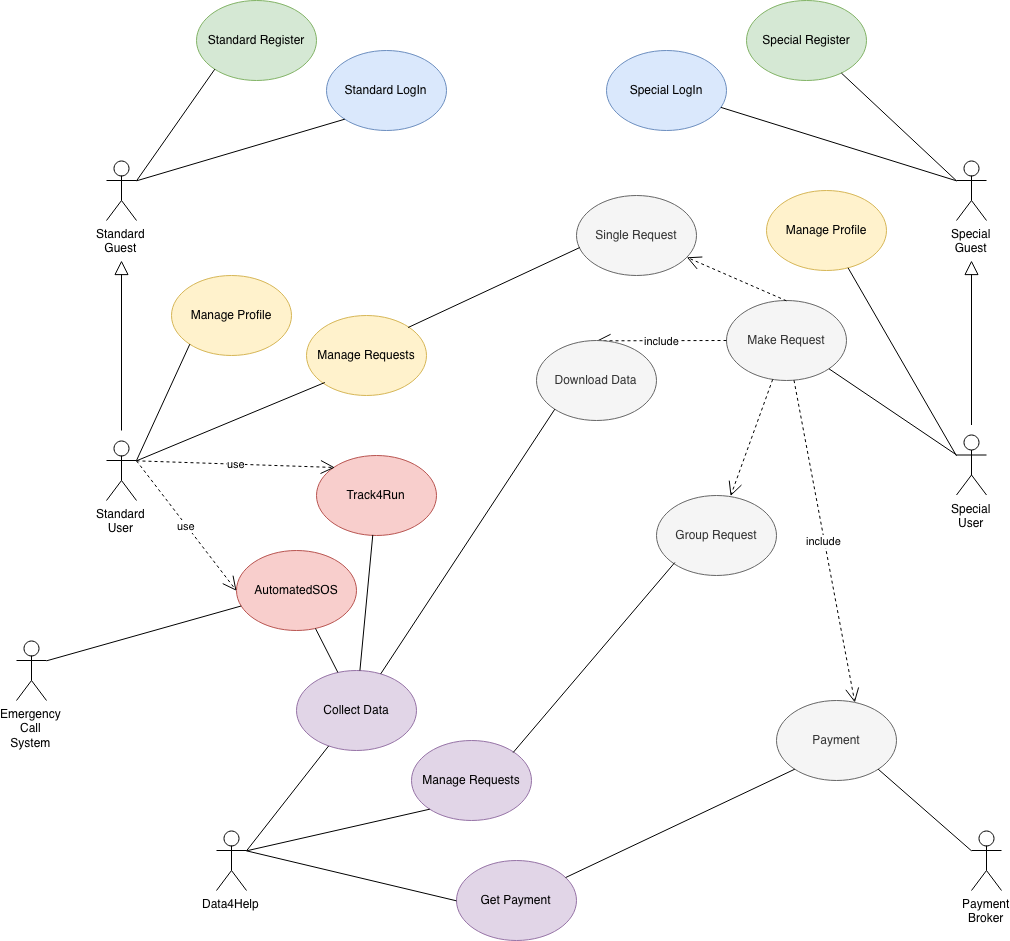
\includegraphics[width=\textwidth]{img/UseCase_Diagram.png}
  \hspace{0.05\linewidth}
  \centering
  \caption{Use Case Diagram}
  \label{img:UseCase_Diagram}
\end{center}
\end{figure}

\section{User Characteristics}
Those applications have different targets.

\subsubsection{AutomatedSOS}
This mobile app is thought for elderly people. It is not necessary that the user is a “tech addicted” because a familiar can setup the system for him/her and than it will work autonomously.

\subsubsection{Track4Run}
This mobile app is thought for athletes. It is most dedicated to young people who use frequently tech products.

\subsubsection{Third party WebApp}
This application is thought for companies who want to analyse data collected by the app. They could be statistics or pharmaceutical companies, hospitals, etc.

\section{Constraints}

\subsection{Anonymous data collection}
Companies who want to analyse data from a group of people without asking the permission to every single person must make a request for anonymized data of a group of at least 1000 people.

\subsection{Privacy}
Before allowing a company to access to user’s data, it is necessary to get a formal permission by the user.

\subsection{Regulatory Policies}
When a new user registers to the service he must accept the privacy policy in order to use the application.
He must be informed about personal and sensible data collection that is carried out by the applications (his/her position and his/her health parameters).
%%In every moment the user can ask TrackMe to delete all the collected data about him.
All the collected data must be kept safe and must not be accessible by unauthorized person.
Also, third parties who access the service must guarantee the security of the data.
The whole process must comply with the GDPR regulations for the protection of users' personal data.
\clearpage

\subsection{Hardware limitations}\label{hardwareLimitation}
In order to use the service, user’s hardware should comply to these minimum requirements:
\subsubsection{Mobile application}
\begin{itemize}
  \item Smartphone:
  \begin{itemize}
    \item iOS or Android operative system;
    \item UMTS/4G Internet connection with a minimum speed of 1Mb/s;
    \item Bluetooth antenna;
    \item GPS antenna;
    \item 300 Mb available memory;
    \item Dual-core processor;
    \item 1 Gb RAM.
  \end{itemize}
  \item Smartwatch / other health device:
  \begin{itemize}
    \item Bluetooth antenna;
    \item Heartbeat sensor;
    \item Pressure sensor.
  \end{itemize}
\end{itemize}

\subsubsection{Web application}
\begin{itemize}
  \item Computer:
  \begin{itemize}
    \item Internet connection with a minimum speed of 1Mb/s;
    \item Browser application;
    \item 720p monitor resolution.
  \end{itemize}
\end{itemize}

\subsection{Parallel operation}
The system must guarantee the operation of the system in case of simultaneous use of the mobile app by at least 100,000 users and simultaneous use of the web app by at least 10,000 users.
Consequently, the DBMS must be able to process a large number of simultaneous transactions.

\subsection{Reliability requirement}
The system reliability, seen as the probability that components and performances will meet the requirement during a specified period of time, must be at least 95\%.

\subsection{Availability requirement}
The system should be available 24/7 in order to guarantee the services and manage emergency situations.

\subsection{Criticality of the system}
\subsubsection{AutomatedSOS}
An error in the system could result in an unnecessary call for an ambulance or in a failure to call an ambulance.
\subsubsection{Track4Run}
An error in the system could cause a non-optimal use of the service.

\section{Assumptions and Dependencies}
From now on the following assumptions are given for guaranteed:
\begin{enumerate}
  \item Users of the app have a phone with an iOS or Android operating system;
  \item Users of the app have a phone with working GPS module with an uncertain of \begin{math} \pm1 \end{math} meter;
  \item All users enjoy a stable Internet connection;
  \item Users accept or refuse a request for access to their data within 24 hours from when it has been recievd. After this period the request is considered rejected;
  \item Each user is identified with his/her/its e-mail;
  \item Once a request is accepted by a user, the system provides the applicant with the required data within 24 hours;
  %%\item Users enter the correct data during registration.
  \item The user autonomously recharges the smartphone and the smartwatch when its battery is low;
  \item A user cannot participate in two races at the same time;
  \item Every request for access to user's personal data from a third parties must be explicitly accepted by the user;
  \item When a third party accesses to the personal data of a user it is responsible for any unauthorized disclosure of data.
\end{enumerate}

\vspace{1cm}

Behavioural during devices recharge time:
\begin{enumerate}
  \item If the smartphone is charging in a fixed position near the user, the wearable device remains connected via Bluetooth to the smartphone and the \textit{AutomatedSOS} service is not interrupted;
  \item If the smartphone is charging in a fixed position, the \textit{Track4Run} service is interrupted;
  \item If the smartphone is charging using a transportable battery, all the services keep working;
  \item If the wearable device is charging, the service \textit{AutomatedSOS} is interrupted;
  \item If the wearable device is charging, the service \textit{Track4Run} keep working (available only data about position);
\end{enumerate}

\section{Future Extensions}
The addition of new features will be evaluated in the future. The possible proposals are:
\begin{enumerate}
  \item The creation of a new application with the purpose of collecting user data, without offering services such as \textit{AutomatedSOS} and \textit{Track4Run}. Users will be paid to use the application consistently. This operation considerably increases the number of users and also collects data from those subjects that are currently excluded (people who are not elderly and do not practice sports);
  \item The possibility for the user to share their sanitary facilities for free with their doctor.
\end{enumerate}
